%=========================================================================
% (c) 2011, 2012 Josef Lusticky <xlusti00@stud.fit.vutbr.cz>

\chapter{Introduction}
Today we live in a world where embedded systems are part of almost every electronic device.
Modern television contains embedded systems to allow you to browse web,
modern cars contain embedded systems to give you summary information
about the journey using GPS, even fridge showing the list of things you plan to buy at a market are becoming popular.
Embedded systems are becoming spread more than ever and so does
their need for a network connection.

Contiki is an operating system targeted at embedded systems
developed by Adam Dunkels at Swedish Institute of Computer Science in Kista, Sweden.
Contiki brings new concepts to the embedded world such as Protothreads and features
the Internet Protocol version 6 and 4 support.
Since Contiki aims for maximum portability it is written in C programming language.
Contiki therefore provides an ideal solution for connecting
embedded systems to existing network on many different hardware platforms.

Time synchronisation is also important today.
Almost every modern system has a need for an exact time -
your video-recorder or home cinema automatically recording film at specified time, your washing-machine finishing the
desired program when you go back home or your radio automatically adjusting its clock when the time changes
due to daylight saving.

Network Time Protocol (NTP) is ubiquitous protocol for time synchronisation between computers on modern Internet.
Though being one of the oldest protocol, NTP is still developed and updated to conform to the latest
network standards. Actual version at the time of writing is NTP version~4, which updates its previous version to
accommodate the Internet Protocol version~6.

This thesis describes Contiki operating system, its concepts and philosophy,
Network Time Protocol version~4 and design and implementation of NTP client for Contiki operating system.


%=========================================================================
% (c) 2011, 2012 Josef Lusticky <xlusti00@stud.fit.vutbr.cz>

\chapter{Contiki OS}
Only 2\% of all microprocessors that are sold today are used in PCs and the remaining 98\%
of all microprocessors are used in embedded systems~\cite{thesis-programming}.
%! MCU DOES NOT HAVE MEMORY
The microprocessors used in embedded systems have much smaller amounts of memory than PC computers.
Moore's law predicts that these devices
can be made significantly smaller and less expensive in the future.
While this means that embedded system networks can
be deployed to greater extents, it does not necessarily imply
that the resources will be less constrained~\cite{paper-contiki}.
The memory constraints make programming for embedded systems a challange.

Operating system Contiki is targeted at embedded systems supporting MSP430, AVR, ARM, x86
architectures and many others~\cite{contiki-docs}.
Contiki aims for maximum portability and therefore is written in C.
It is a feature-rich operating system and it
is possible to describe only some of its features in this thesis.
%! WE WILL

Contiki OS features lightweight stackless threads called Protothreads.
Protothreads are a new concept brought to the embedded world by Contiki,
they are extremely lightweight and compatible with standard C~\cite{paper-protothreads}.
Each Protothread does not require a separate stack which fits them perfectly
for usage in memory constrained embedded systems.
Protothreads are more detailed discussed in section~\ref{sec:contiki-protothreads}.

Contiki also features TCP/IP communication stack called uIP~(micro~IP)
that comforms to Request For Comments memorandums published by the Internet Engineering Task Force.
The uIP provides communication abilities using both IPv4 and IPv6~\cite{contiki-docs}.
Contiki with its uIP stack is IPv6 Ready Phase 1 certified
and therefore has the right to use the IPv6~Ready silver logo~\cite{ipv6ready-db}.
Before Contiki's uIP the embedded world considered IP to be too heavyweight.
That means all earlier IP implementations for general purpose computers
were much bigger than the memory constrained embedded systems could use~\cite{interconnecting}.
The communication stack uIP is closely described in section~\ref{sec:contiki-uip}.

Next to the uIP, Contiki is equipped with other communication stack called Rime.
Rime is a layered communication stack for sensor networks,
with much tinner layers than traditional architectures~\cite{paper-rime}.
Rime is designed to simplify the implementation of communication
protocols on low-power radios.
The communication primitives in the Rime stack were choosen
based on what typical sensor network protocols use -
single-hop unicast, single-hop broadcast or multi-hop~\cite{contiki-docs,paper-rime}.

Beside Protothreads and communication stacks uIP and Rime,
Contiki contains very simple, relatively small and easy to use filesystem
called Coffee Filesystem (CFS),
graphical user interface called Contiki Toolkit (CTK),
Executable Linkable Format (ELF) loader for loading object files into a running Contiki system
and much more.

Operating system Contiki, uIP and Protothreads are used by hundreds of companies in embedded devices in
such diverse systems as car engines, oil boring equipment, satellites, and container security systems~\cite{thesis-programming}.
The software is also used both in academic research
projects and in university project courses on embedded systems throughout the
world.

Contiki is developed by a group of developers from industry and academia
lead by Adam Dunkels from the Swedish Institute of Computer Science.
The Contiki team currently consists of sixteen developers from SICS,
SAP AG, Cisco, Atmel, NewAE and TU Munich~\cite{contiki-docs}.
Contiki is also deployed at RheinMain University in Wiesbaden.
The 3-clause BSD license is placing minimal restrictions on how Contiki can be redistributed.
Contiki version 1.0 was released in 2002, version 2.0 in 2007 and the latest version
at the time of writing was 2.5 released in 2011.
The actual development happens in online repository accessible on Contiki homepage at \url{http://www.contiki-os.org/}
using Git version control system.

\begin{figure}
  \centering
  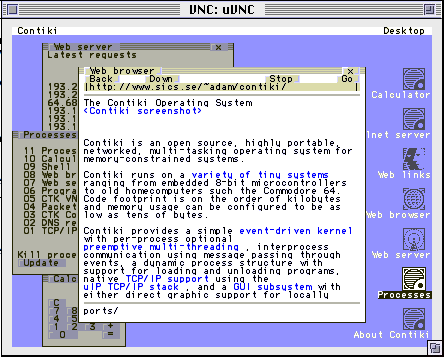
\includegraphics[width=9cm,keepaspectratio]{fig/contiki-vnc.png}
  \caption{Screenshot of running Contiki OS with CTK}
  \label{fig:contiki}
  \bigskip
\end{figure}


%=========================================================================
% (c) 2011, 2012 Josef Lusticky <xlusti00@stud.fit.vutbr.cz>

\section{Protothreads}\label{sec:contiki-protothreads}
Protothreads provide a way to run C functions quasi-paralelly, that is, a C functions work in a way similiar to thread.
In Contiki Protothreads allow process to wait for incoming events. While waiting for an event to occur another function
can be run. The core of this solution is C switch statement used in conjuction with variable (called local continuation)
containing the position where the function was interrupted. Next time function continues from this point.

The advantage of Protothreads over ordinary threads is that a Protothread does not require a separate stack.
In memory constrained systems, the overhead of allocating multiple stacks can consume large amounts of
the available memory. In contrast, each Protothread only requires few bytes for storing the state of execution.

A Protothread is driven by repeated calls to the function in which the Protothread is running.
Each time the
function is called, the Protothread will run until it blocks or exits.
Protothreads are implemented using local continuations. A local continuation represents the current state
of execution at a particular place in the program, but does not provide any call history or local variables.

The Protothreads API consists of four basic operations: initialization (PT\_INIT()), execution (PT\_BEGIN()),
conditional blocking (PT\_WAIT\_UNTIL()) and exit (PT\_END()). On top of these, two convenience functions
are built: reversed condition blocking (PT\_WAIT\_WHILE()) and Protothread blocking (PT\_WAIT\_THREAD())~\cite{paper-protothreads}.

To understand how are Protothreads implemented and how do the actually work please refer
to appendix~\ref{app:protothreads} in which an example of usage is shown.

Since Protothreads are implemented using standard C, library providing Protothreads can be used everywhere C toolchain is available.
But there are some cons to consider. Because protothreads are stackless, a Protothread can only run within a single C function.
There is also no way of storing automatic local variables. And since Protothreads are implemented using C {\it switch} statement, and these can
not be nested, the code that uses Protothreads cannot use {\it switch} statements itself.
Workaround for storing local variables is to prepend them with the {\it static} keyword, which make them being put into data segment
by compiler and thus remembering the value between the function calls.


%=========================================================================
% (c) 2011, 2012 Josef Lusticky

\section{uIP}\label{sec:contiki-uip}
The TCP/IP protocol suite is often used for communication over the Internet as well as local networks.
uIP (micro IP) is a complete TCP/IP communication stack developed by Adam Dunkels
for memory constrained systems such as embedded systems.

Before uIP, the TCP/IP architecture was considered to be heavyweight
due to its perceived need for processing power and memory.
The IP protocol was seen as too large to fit into the constrained environment -
existing implementations of the IP protocol family for general purpose computers would need hundreds
of kilobytes, whereas a typical constrained system has only a few tens of kilobytes of memory~\cite{interconnecting}.
For this reason, several non-IP stacks were developed.

In the early 2000's, however, this view was challenged by lightweight implementations of the IP
protocol family for smart objects such as the uIP stack~\cite{interconnecting}.
uIP showed that the IP architecture would fit nicely into the typical constrained systems,
without removing any of the essential mechanisms from IP.
Note that these resources, which are considered constrained today, are fairly close to the
resources of general purpose computers that were available when IP was designed~\cite{interconnecting}.
Since its initial release, the uIP stack has become widely used in networked
embedded systems~\cite{interconnecting, thesis-programming}.

uIP provides two different application programming interfaces to programmers:
a BSD sockets-like API called Protosockets and raw event-driven API.
Protosockets are based on Protothreads putting the same limitation on them - such as
no way of storing automatic local variables and an impossibility of using the C {\it switch} statement.
Protosockets only work with TCP connections~\cite{contiki-docs}.
Since NTP uses UDP, Protosockets will not be further
discussed in this thesis. For more information about Protosockets
please refer to the Contiki documentation~\cite{contiki-docs}.

uIP contains only the absolute minimum of required features to fulfill the protocol standard.
It can only handle a single network interface and contains the IP, ICMP, UDP and TCP protocols~\cite{contiki-docs}.
In order to reduce memory requirements and code size,
the uIP implementation uses an event-based API, which is fundamentally different
from the most common TCP/IP API, the BSD sockets API, present on Unix-like systems
and defined by the POSIX standard~\cite{thesis-programming,posix}.
An application is invoked in response to certain events and
it is up to the application that is receiving events from uIP to handle all
work with data to be transmitted. E.g. if the data is lost in the network,
the application will be invoked and then has to resend the data.
This approach is based on the fact that it should be simple for the application
to rebuild the same data.
This way, the uIP stack does not need to use explicit dynamic memory allocation.
Instead, it uses a single global buffer for holding packets and has a fixed
table for holding the connection state.
The global packet buffer is large enough to contain one packet of maximum size~\cite{contiki-docs}.

When a packet arrives from the network, the device driver places it in the
global buffer and calls the TCP/IP stack.
If the packet contains data, the TCP/IP stack will notify the corresponding application.
Because the data in the buffer will be overwritten by the next incoming packet,
the application will either have to act immediately on the data or copy the data into
its own buffer for later processing.
The packet buffer will not be overwritten by new packets before the application has processed the data~\cite{contiki-docs}.
Packets that arrive when the application is processing the data must be queued,
either by the network device or by the device driver.
That means uIP relies on the hardware when it comes to buffering.
Most single-chip Ethernet controllers have on-chip buffers
that are large enough to contain at least 4 maximum sized Ethernet frames~\cite{contiki-docs}.
This way, uIP does not have to have its own buffer structures and thus
only a minimal memory amount is required.
Possible packet loss is a trade-off for minimalism and ability to communicate using TCP/IP.
It is not such a big deal for communication using TCP on the transport layer
because of the acknowledgement scheme used in TCP to prevent data loss.
However data carried on UDP can be irrecoverably lost.

As was expected, measurements show that the uIP implementation provides very low
throughput, particularly when communicating with a PC host~\cite{thesis-towards}.
However, small systems that uIP is targeting, usually do not produce enough data
to make the performance degradation a serious problem~\cite{thesis-towards}.

Despite being so small, uIP is not only RFC compliant, but also IPv6 Ready Phase 1 certified.
uIP is written in the C programming language and it is fully integrated with the Contiki operating system.
In uIP, there are even some more tricks to shrink the stack
but complete uIP description is outside the scope of this thesis.
Please refer to the Contiki documentation for more details~\cite{contiki-docs}.


%=========================================================================
% (c) 2011, 2012 Josef Lusticky

\section{Kernel and processes}\label{sec:contiki-kernel}
The kernel in Contiki is event-driven providing cooperative multitasking
environment, but the system supports preemptive
multithreading that can be applied on a per-process basis~\cite{video}.
The preemption is not implemented in the kernel, but
preemptive multithreading is implemented as a library that is linked only with programs that
explicitly require multithreading~\cite{paper-contiki}.
The kernel itself contains no platform specific code, it implements only CPU multiplexing and
lets device drivers and applications communicate directly with hardware~\cite{video}.

From high level of abstraction,
applications in Contiki OS are implemented and run as processes.
Protothreads, the lightweight threads described in section~\ref{sec:contiki-protothreads},
are used in Contiki to implement processes.
Both the Contiki kernel and Contiki applications use
Protothreads extensively to achieve cooperative multitasking~\cite{contiki-wiki-faq}.
Every Contiki process consists of a process control block and a process thread~\cite{contiki-wiki-processes}.
The process control block contains run-time information about the process and
the process thread contains the code of the process.
Among other things, the process control block contains
textual name of the process, pointer to the process thread and state of the process.
The process thread is implemented as a single Protothread,
that is invoked from the process scheduler in the Contiki kernel~\cite{contiki-wiki-processes}.

From low level of abstraction,
every application is implemented as a simple C function
and the process control block remembers the actual state of execution of this function
in the same way as the local continuation works by Protothreads.
Processes are therefore running quasi-parallely in Contiki.

\bigskip
\begin{lstlisting}[caption=Process control block in Contiki OS]
struct process {
	struct process *next;
	const char *name;
	int (* thread)(struct pt *, process_event_t, process_data_t);
	struct pt pt;
	unsigned char state, needspoll;
	};
\end{lstlisting}

Process control block is not declared or defined directly,
but through the {\it{PROCESS()}} macro.
This macro takes two parameters: the variable name of the process control block
and a textual name of the process,
which is used in debugging and when printing out lists of active processes to users~\cite{contiki-wiki-processes}.

All code execution is initiated by the Contiki kernel
that acts like a simple dispatcher calling these functions~\cite{contiki-docs}.
Just like Protothreads, processes are also implemented using macros,
making them fully standard C compatible.

In Contiki, code run in either of two execution contexts:
cooperative, in which code never preempts other code, and preemptive,
which preempts the execution of cooperative code and returns control
when preemptive code is finished.
Processes always run in cooperative mode,
whereas interrupt service routines and real-time timers run in preemptive mode~\cite{contiki-wiki-processes}.
Code running in both execution contexts illustrates figure~\ref{fig:contiki-execution-context}.

\begin{figure}
  \centering
  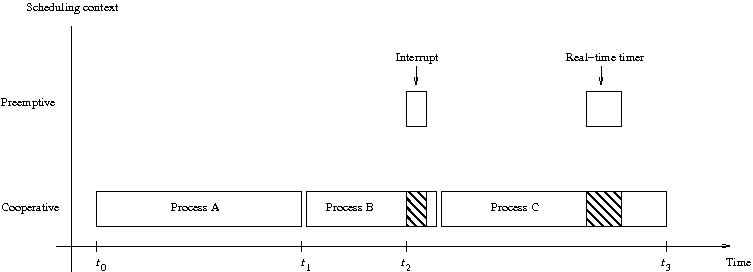
\includegraphics[width=13cm,keepaspectratio]{fig/Execution-contexts.png}
  \caption{Contiki execution contexts by A. Dunkels}
  \label{fig:contiki-execution-context}
\end{figure}

Interprocess communication is done by posting events in Contiki OS -
processes communicate with each other by posting events to each other~\cite{paper-contiki}.
There are two types of events: synchronous and asynchronous.
Synchronous events are directly delivered to the receiving process when posted and
can only be posted to a specific processes~\cite{contiki-wiki-processes}.
Because synchronous events are delivered immediately,
posting synchronous event is equivalent to a function call:
the process to which an event is delivered is directly invoked,
and the process that posted the event is blocked
until the receiving process has finished processing the event~\cite{contiki-wiki-processes}.

Asynchronous events are delivered to the receiving process
some time after they have been posted~\cite{contiki-wiki-processes}.
Before delivery, the asynchronous events are held on event queue inside Contiki kernel.
The kernel loops through this event queue and delivers
the event to the process by invoking the process. 
The receiver of an asynchronous event can be either a specific process
or all running processes~\cite{contiki-wiki-processes}.

%! paper-contiki - dunkels04contiki
%Being able to power down the device
%when the network is inactive is often required way to reduce energy consumption.
%Power conservation mechanisms
%depend on both the applications and the network protocols.
%The Contiki kernel contains no explicit power
%save abstractions, but lets the the application specific parts
%of the system implement such mechanisms.
%To help the application decide when to power down the system, the event
%scheduler exposes the size of the event queue.
%This information can be used to power down the processor when there
%are no events scheduled.
%! paper-contiki

%As stated before, Contiki is well documented and you can find out more about
%the kernel as well as the system in the documentation~\cite{contiki-docs}.


%=========================================================================
% (c) 2011, 2012 Josef Lusticky

\section{Timers}\label{sec:contiki-timers}
The Contiki kernel does not provide support for timed events,
instead an application that wants to use timers needs to explicitly use a timer library.
The timer library provides functions for setting, resetting and restarting timers,
and for checking if a timer has expired.
An application must manually check if its timers have expired - this is not done automatically~\cite{contiki-docs}.

Contiki has one clock library and a set of timer libraries: timer, stimer, ctimer, etimer, and rtimer~\cite{contiki-wiki-timers}.
The clock library provides functionality to handle the system time and to block the CPU for short time periods.
It is the interface between Contiki and the platform-specific hardware clock~\cite{contiki-docs}.
The timer libraries are implemented with the functionality of the clock library as a base~\cite{contiki-wiki-timers}.

The timer and stimer libraries provide the simplest form of timers and are used to check whether a time period has passed.
The difference between these two is the resolution of time -
timers use system clock ticks, whose value is incremented when an interrupt from the hardware clock occurs,
while stimers use seconds to offer much longer time periods~\cite{contiki-wiki-timers}.
The value representing seconds is also incremented in the interrupt service routine (ISR),
but only when enough clock ticks since last increment occurred.
The number of clock ticks within one second is represented by the
{\it{CLOCK\_SECOND}} macro provided by the clock library.
That means there are {\it{CLOCK\_SECOND}} interrupts from the hardware clock per second.
The usage of the timer library and {\it{CLOCK\_SECOND}} macro is shown in appendix~\ref{app:protothreads}.

The simplest timer and stimer libraries are not able to post an event when a timer expires.
Event timers should be used for this purpose.
Event timers (etimer library) provide a way to generate timed events.
An event timer will post an event to the process that set the timer when the
event timer expires~\cite{contiki-docs}.
The etimer library is implemented as a Contiki process and uses the timer library as a base.

Callback timers (ctimer library) provide a timer mechanism that calls a specified
C function when a ctimer expires~\cite{contiki-docs}.
Thus, they are especially useful in any code that does not have an
explicit Contiki process~\cite{contiki-wiki-timers}.

The Real-time timers (rtimer library) handle the scheduling and execution of
real-time tasks with predictable execution times~\cite{contiki-docs}.
The rtimer library provides real-time task support through callback functions -
the rtimer immediately preempts any running Contiki process in order to let the real-time tasks
execute at the scheduled time~\cite{contiki-wiki-timers}.
This behaviour is illustrated in figure~\ref{fig:contiki-execution-context}.
The rtimer library uses a separate hardware clock
to allow a higher clock resolution~\cite{contiki-wiki-timers}.
The small part of the rtimer library is architecture-agnostic,
but the particular implementation is platform-specific.



%=========================================================================
% (c) 2011, 2012 Josef Lusticky <xlusti00@stud.fit.vutbr.cz>

\chapter{Network Time Protocol}
Network Time Protocol provides mechanism for synchronising systems' clocks over the variable-latency data network.
% packet-oriented + citation
NTP was introduced and is still developed by David Mills at University of Delaware in Newark, United States.
NTP is argueably the longest running, continuously operating,
ubiquitously available protocol in the Internet~\cite{ntp-overview}.
Despite being one of the oldest surviving protocol on the Internet, it is not old-fashioned at all.
NTP version 4 described in RFC~5905~\cite{rfc5905} is an update to older NTPv3 to accomodate NTP to IPv6.
Version 4 also includes improvements in
the mitigation and discipline algorithms that extend
the potential accuracy to the tens of microseconds with modern
workstations and fast LANs~\cite{rfc5905}.
NTPv4 corrects some
errors in NTPv3 design and includes optional extension mechanism
that can be used for adding more capabilites to NTP, e.g. the
Autokey security protocol described in RFC~5906
for authenticating servers to clients.

Simple Network Time Protocol is simplified NTP implementation lacking complex
synchronisation algorithms used by NTP.
%citation  ?? ~\cite{rfc5905} ??
SNTP is also described in RFC 5905.
The packet of SNTP has the same structure and content as packet of NTP~\cite{rfc5905}.
From observing the network communication one can not tell whether the client
is full blown NTP implementation or just SNTP.
SNTP is a simplified sub-set of the algorithms used by the NTP protocol
making the client implementation not only easier, but also suitable for
resource constraint systems such as embedded systems.


%=========================================================================
% (c) 2011, 2012 Josef Lusticky

\section{Topology and hierarchy}\label{sec:ntp-topology}
NTP uses two different communication modes:
one to one, referred as unicast mode, and one to many, referred as broadcast mode~\cite{rfc5905}.
In unicast communication mode, NTP client sends request and NTP server sends response.
In broadcast communication mode, the client sends no request
and waits for a broadcast message from one or more servers~\cite{rfc5905}.

NTP servers are rated with stratum (plural form strata) number which represents their position
in an NTP hierarchy and their possible accuracy~\cite{rfc5905}.
Primary (stratum 1) servers synchronise to the reference clock directly traceable to UTC via
radio, satellite or modem.
The stratum 2 servers synchronise to stratum 1
servers via hierarchical subnet.
The stratum 3 servers synchronise to stratum 2 servers, and so on.
The maximum stratum is 15, number 16 means unsynchronised server
and higher numbers (up to 255) are reserved~\cite{rfc5905}.
Synchronisation between servers in the same stratum level is also possible.
Figure~\ref{fig:ntp-hierarchy} shows a brief hierarchy of NTP.
\begin{figure}
  \centering
  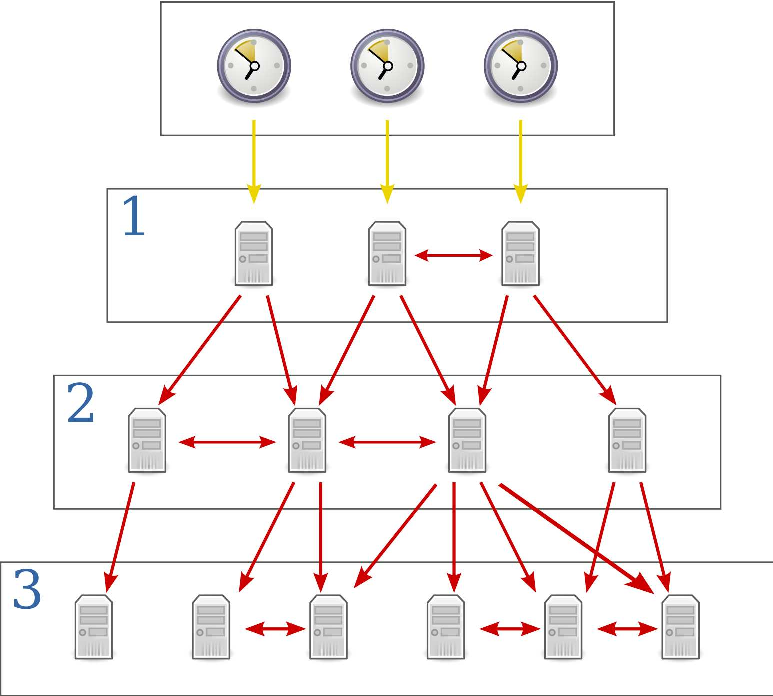
\includegraphics[width=9cm,keepaspectratio]{fig/Network_Time_Protocol_servers_and_clients.pdf}
  \caption{Topology and hierarchy of NTP by B. Esham}
  \label{fig:ntp-hierarchy}
  \bigskip
\end{figure}


%=========================================================================
% (c) 2011, 2012 Josef Lusticky <xlusti00@stud.fit.vutbr.cz>

\section{Time and timescales}\label{sec:ntp-time}
For expressing the time NTP always uses the Coordinated Universal Time (UTC)~\cite{rfc5905}.
UTC is maintained by the International Bureau of Weights and Measures in Paris, France.
It is the time scale that forms the basis for coordinated dissemination
of standard frequencies and time signals~\cite{bipm-utc}.
The time specified by UTC is the same for all timezones.
Its calculation is the same as with Greenwich Mean Time (GMT),
however the daylight savings are not accounted.

The UTC scale is adjusted by the insertion of leap seconds to ensure approximate
agreement with the time derived from the rotation of the Earth~\cite{bipm-utc}.
The atomic clocks, on which UTC is based, are so precise that
they do not match the rotation of the Earth,
which periodically speeds up and slows down due to the action
of tides and changes within the Earth's core~\cite{cnn-earth}.
The goal of a leap second is to catch up UTC with these changes.
The leap second is inserted or deleted on the advice of
International Earth Rotation and Reference Systems Service~\cite{bipm-utc}.
NTP is well designed for leap second occurrence -
there is Leap Indicator field
in the structure of NTP packet and there are also fields intended for
information about leap second in structures that NTP algorithm uses~\cite{rfc5905}.
The formal definition of UTC does not permit double leap seconds~\cite{posix}.

In computer the system time is represented by system clock maintained by
hardware and operating system.
The goal of the NTP algorithms is to minimize
both the time difference and frequency difference between UTC and the system clock.
When these differences have been reduced below nominal
tolerances, the system clock is said to be synchronised to UTC~\cite{rfc5905}.
It has never been a goal of NTP to take care of local time,
it is up to operating system to provide user the correct local time~\cite{ntp-overview}.

The NTP and POSIX timescales are based on the UTC timescale,
but not always coincident with it~\cite{ntp-leap}.
Both timescales reckon in seconds since the prime epoch,
but the origin of the NTP timescale, the NTP prime epoch, is 00:00:00 UTC on 1 January 1900,
while the prime epoch of the POSIX timescale is 00:00:00 UTC on 1st January 1970~\cite{ntp-leap}.
%! VYHODIT?
So upon the first tick of POSIX clock on 1st January 1970 the NTP clock read 2~208~988~800,
representing the number of seconds since the NTP prime epoch.
Some of interesting dates with their respective NTP time values
can be found in appendix~\ref{app:dates}.


%=========================================================================
% (c) 2011, 2012 Josef Lusticky <xlusti00@stud.fit.vutbr.cz>

\section{Network and timestamps}\label{sec:ntp-network}
Network specification of NTP defines that
the protocol uses the User Datagram Protocol (UDP) on port number 123~\cite{ianna-ports,rfc5905}.
Reliable message delivery such as TCP can actually make the delivered NTP packet less reliable since retries
would increase the delay value and other errors~\cite{rfc5905}.
This is mostly due to overhead of communication with TCP on transport layer.

NTP manipulates with the time through timestamps - a record of time.
NTP timestamp has two fields. The seconds field expressing the number of seconds
and the fraction field expressing fraction of a second~\cite{rfc5905}.
All NTP time values are represented in twos-complement format, with
bits numbered in big-endian fashion from zero starting at the left, or high-order, position~\cite{rfc5905}. 
There are two formats of timestamp in NTP packet structure:
long 64-bit and short 32-bit as shown on figure~\ref{fig:ntp-timestamps}.
The 64-bit long timestamp used by NTP consists of a 32-bit unsigned seconds
field spanning $2^{32}$ seconds (aprox. 136 years from 1900 to 2036) and a 32-bit fraction field resolving
$2^{-32}$ seconds (aprox. 232 picoseconds)~\cite{rfc5905}.
The short 32-bit timestamp includes a 16-bit unsigned seconds field
and 16-bit fraction field.

There is one more NTP time format - 128-bit date format.
This format is however not transmitted over the network
and since this 128-bit date format is used where sufficient storage and word
size are available~\cite{rfc5905},
there is practically no need of knowing about this format for embedded systems.
But strictly speaking an NTP timestamp is a truncated NTP date format~\cite{rfc5905}.

\begin{figure}
	\centering
	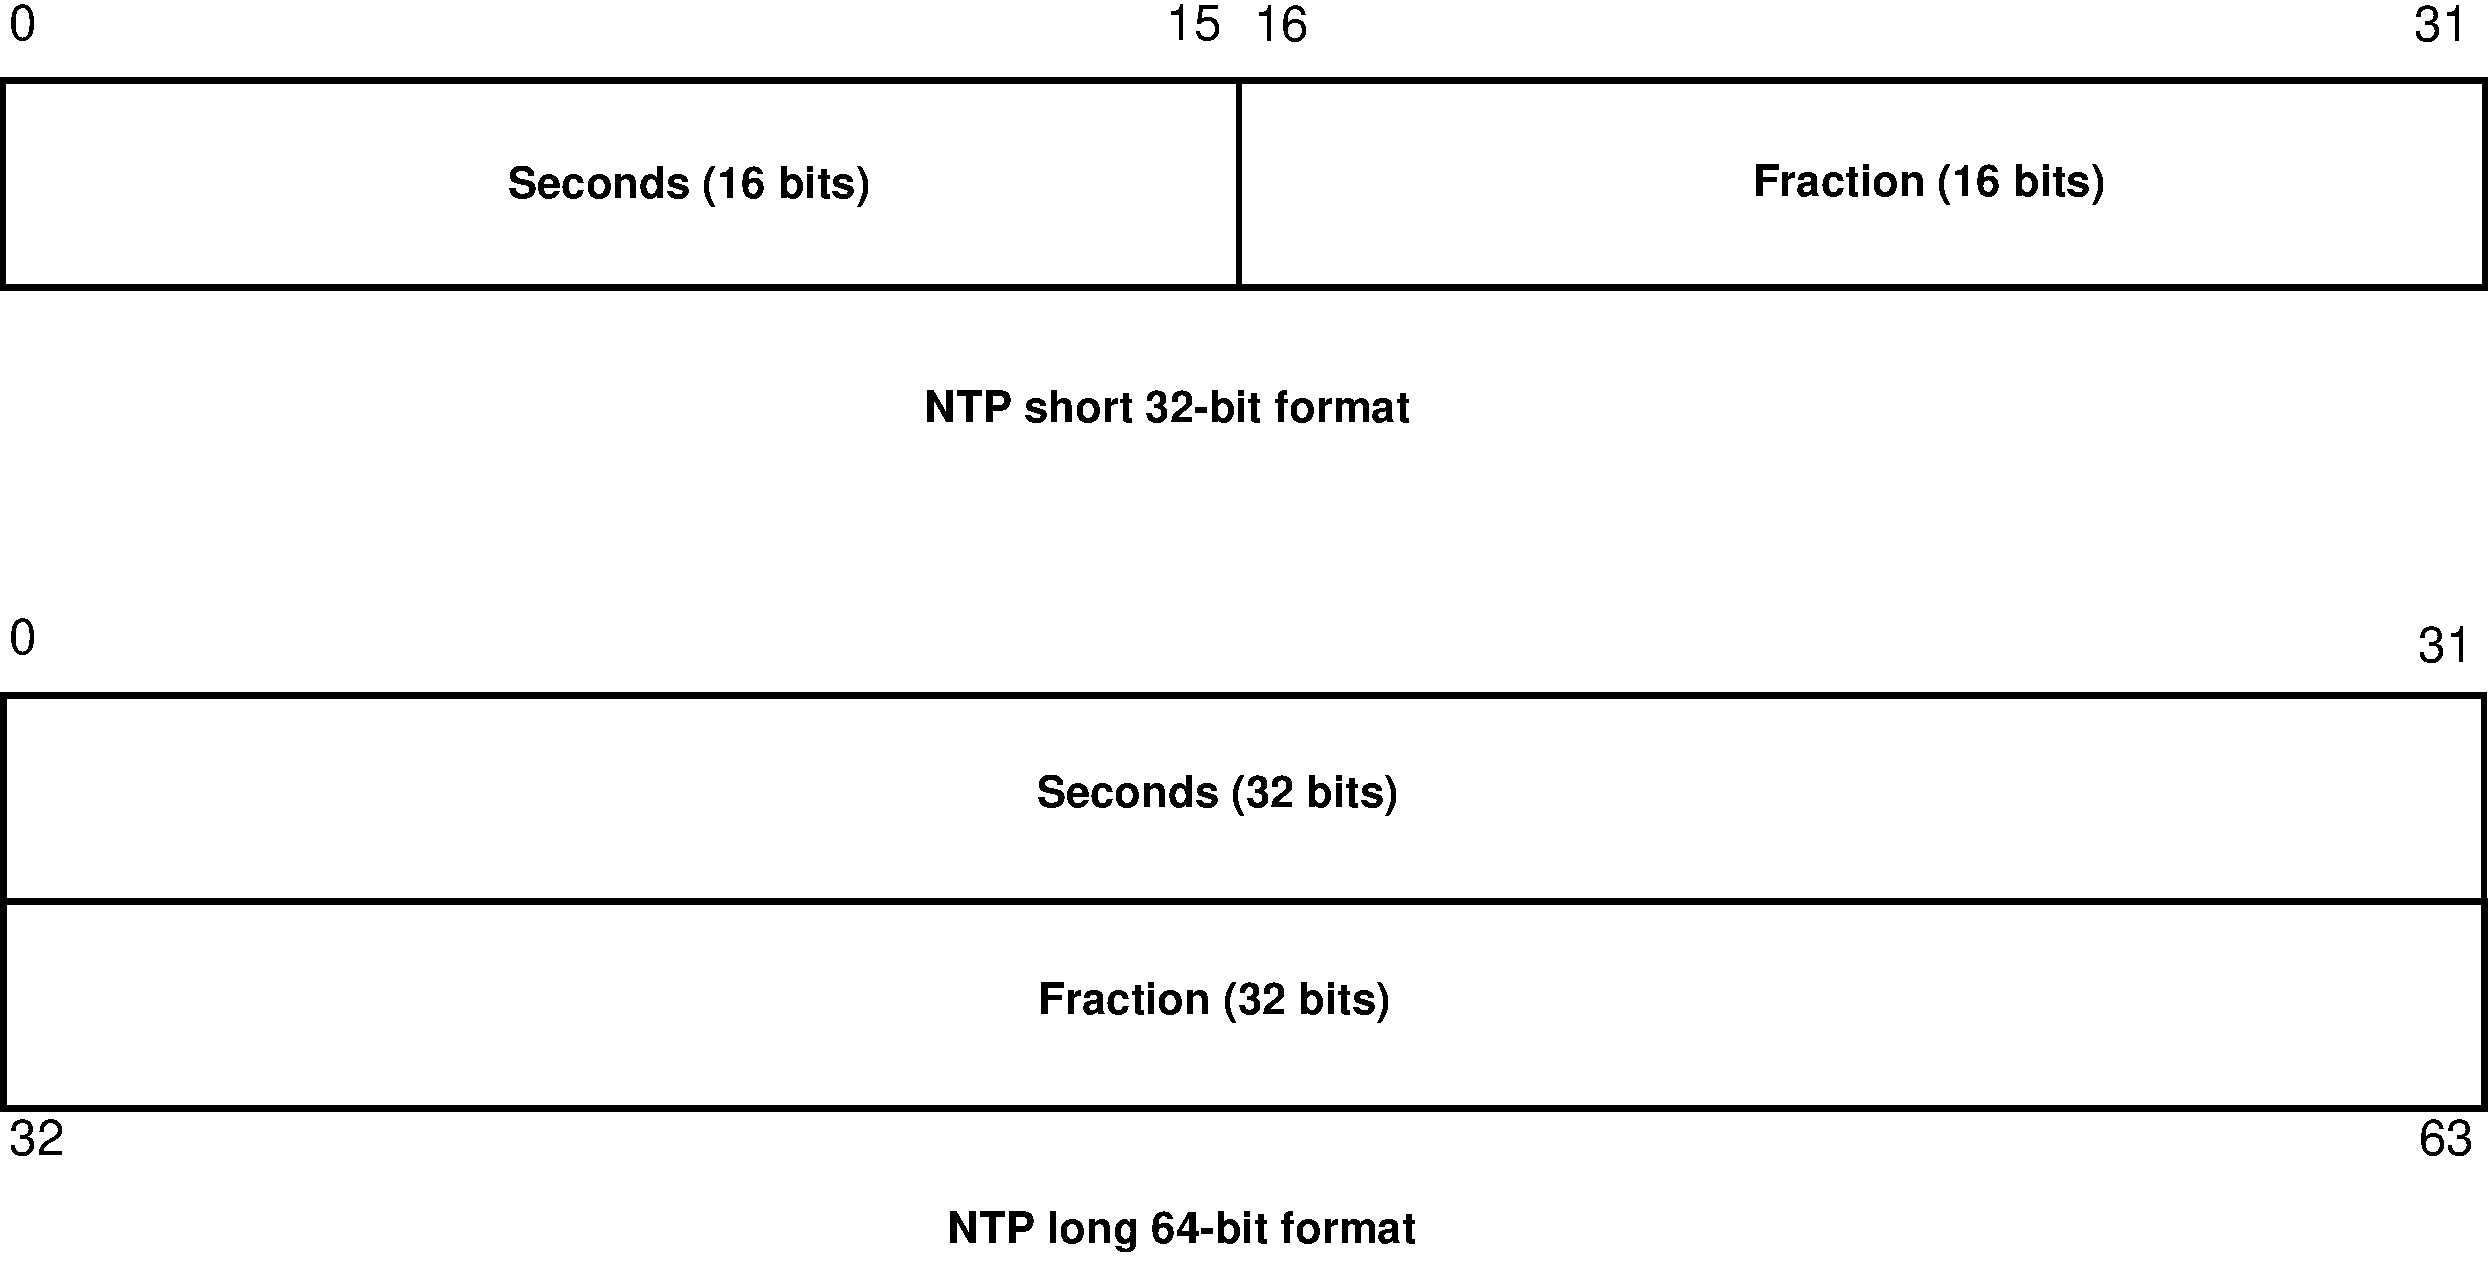
\includegraphics[width=13cm,keepaspectratio]{fig/ntp-timestamps.pdf}
	\caption{Time formats used in NTP packet}
	\label{fig:ntp-timestamps}
	\bigskip
\end{figure}

% TODO - packet

\begin{figure}
	\centering
	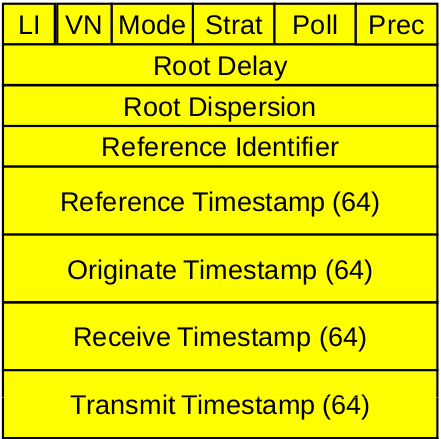
\includegraphics[width=6cm,keepaspectratio]{fig/ntp-packet.png}
	\caption{Basic NTP packet structure}
	\label{fig:ntp-packet}
	\bigskip
\end{figure}


Because the short 32-bit format is used for Root dispersion and Root Delay fields,
they do not need so big scope and precision.
Root dispersion express accumulated total dispersion from primary server
and Root Delay express accumulated roundtrip delay via primary server~\cite{ntp-arch}.

%TODO

Because of network latency the timestamp recieved will never be exactly corresponding to
the current time.
One of the main goals of NTP is to deal with the network latency~\cite{ntp-overview}.



%=========================================================================
% (c) 2011, 2012 Josef Lusticky

\section{Algorithms}\label{sec:ntp-algorithms}
Because of network latency the received Transmit Timestamp will never be exactly
corresponding to the current time.
One of the main goals of NTP is to deal with the network latency~\cite{ntp-overview}.

As described in section~\ref{sec:ntp-network},
there are the following 64-bit long timestamps in NTP packet: Origin, Receive and Transmit Timestamp.
Upon NTP packet arrival, the client determines another timestamp called
Destination Timestamp~\cite{rfc5905}.
This timestamp is represented as T4 on figure~\ref{fig:ntp-client-server}
and is not part of NTP packet structure.

Using these four timestamps, NTP client using unicast communication mode can compute
the local clock offset which is given by $\theta = \frac{1}{2}[(t_2 - t_1) + (t_3 - t_4)]$,
where $t_1$ is the time of the request packet transmission (Origin Timestamp),
$t_2$ is the time of the request packet reception (Receive Timestamp),
$t_3$ is the time of the response packet transmission (Transmit Timestamp) and
$t_4$ is the time of the response packet reception (Destination Timestamp)~\cite{ntp-algor,rfc5905}.
The implicit assumption in the above is that one-way delay is
statistically half of round-trip delay~\cite{rfc5905},
which is given by $\delta = (t_4 - t_1) - (t_3 - t_2)$.

In broadcast communication mode, Origin and Receive Timestamps are not accounted.
The client computes its local clock offset which is given by $\theta = t_3 - t_4$.
The implicit assumption in the above is that one-way delay from server to client is zero.
Since this is never the case, it is useful to provide an
initial volley where the client exchanges several packets with the server in
order to calibrate the propagation delay~\cite{rfc5905}.

When computing the result from more servers, the intersection algorithm is used
for selecting the possible most exact timestamp received from various servers~\cite{ntp-improved-algor,rfc5905}.
Intersection algorithm is derived from Murzollo algorithm but the basic
computation remains the same~\cite{ntp-history}.
First of all a selection of bad and good servers must be made.
Bad servers are called Falsetickers and good are called Truechimers~\cite{rfc5905}.
The division to these sets is based on their response.
As one can assume for a sensible result there must be more Truechimers than Falsetickers~\cite{rfc5905}.

After selecting a set of reliable servers, NTP clock algorithms compute resulting exact timestamp.
The resulting exact timestamp does not have to be the same
as one of those provided by the servers.
NTP clock algorithms calculate using clock accuracy estimates
determined from Root Dispersion, Root Delay and Precision fields of server's response.
These estimates are converted to intervals.
Figure~\ref{fig:ntp-intersection} shows the computation for the following example:
If we have the estimates $10 \pm 2$, $12 \pm 1$ and $11 \pm 1$
then these intervals are $<8; 12>$, $<11; 13>$ and $<10; 12>$ which
intersect to form $<11; 12>$ or $11.5 \pm 0.5$ as consistent with all three values.
The arithmetic mean is used as the result value.
When querying servers again, the algorithm repeats but the new result computation
also depends on the previous result~\cite{rfc5905,ntp-history}.
This eliminates possible jitter which can be caused by repeatedly querying the servers
and getting slightly different answers from them.

\begin{figure}
	\centering
	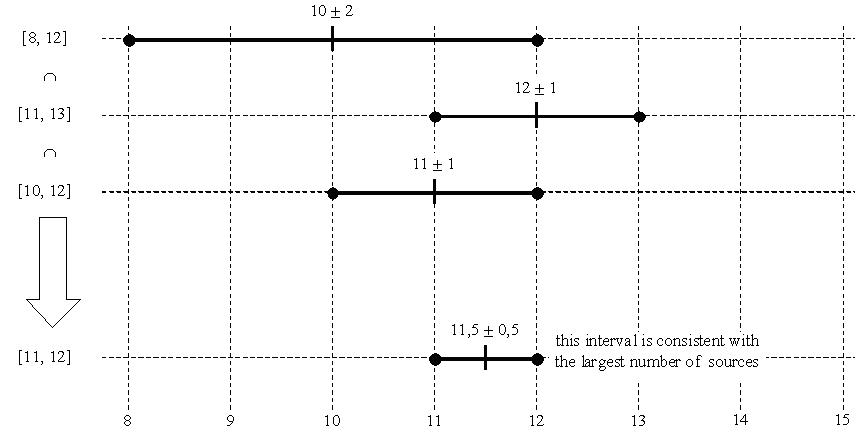
\includegraphics[width=13cm,keepaspectratio]{fig/Marzullo_example-1.jpg}
	\caption{Intersection algorithm by D. Exb}
	\label{fig:ntp-intersection}
	\bigskip
\end{figure}

%Since the clients complying with a subset of NTP, called
%the Simple Network Time Protocol (SNTPv4) [RFC4330], do not need to
%implement the mitigation algorithms ... ~\cite{rfc5905}.



\section{Hardware concerns for implementing real-time support}
A typical desktop computer today includes CPU based on Intel x86 architecture.
Real-Time Clock (RTC) in CMOS memory that is battery powered

Unfortunately Intel x86 architecture is heavily influenced by backwards compatibility,
e.g. the time value can also be stored in Binary Code Digit (BCD) encoding in RTC.

In year 19xx / Starting with Intel 386
Intel introduced
PIT Intel 8253 and 8254 - 3 counters (counter 0 interrupt to OS)


Used by historic versions of Linux
=> read initial time from RTC, setup PIT and interrupts (IRQ 0, INT 8), increment jiffies on every interrupt, provide app resolution of jiffies

init/main.c - time\_init() - read from RTC and save to startup\_time
kernel/sched.c - sched\_init() = PTI setup for interrupts - LATCH (1193180/HZ)
kernel/system\_call.s - timer\_interrupt() in assembly - increments jiffies

The current real time is provided by CURRENT\_TIME (startup\_time+jiffies/HZ) => since jiffies is integer and HZ is 100 => resolution of 10ms.
kernel/sys.c - sys\_time() - CURRENT\_TIME returned


\section{NTP on POSIX-compliant systems}
Operating systems
Linux
OpenBSD
DragonflyBSD

NTP implementations
NTP from ntp.org project - reference implementation
Chrony
OpenNTPD - OpenBSD
dntpd - DragonflyBSD



%=========================================================================
% (c) 2011, 2012 Josef Lusticky <xlusti00@stud.fit.vutbr.cz>

\chapter{Hardware support for real-time}
%! TODO
TODO: Distinguish between TIME and CLOCK

%We need clock~\cite{timecounters}.
\begin{figure}
	\centering
	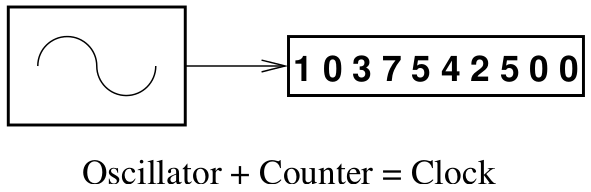
\includegraphics[width=6cm,keepaspectratio]{fig/clock.png}
	\caption{Clock by P. Kamp}
	\label{fig:hw-clock}
	%\bigskip
\end{figure}

A computer clock is an electronic device that counts oscillations in a
quartz crystal with a particular frequency~\cite{thesis-sync}.
These clocks are essentially timers.
The timer counts the oscillations of the crystal, which is associated with
a counter register and a holding register.
For each oscillation in the crystal, the counter is decremented by one.
When the counter becomes zero, an interrupt is generated and the
counter is reloaded from the holding register.
Therefore, it is possible to
program a timer to generate an interrupt by setting an appropriate value in
the holding register, where each interrupt is called a clock tick.
At each clock tick,
the interrupt procedure increments the clock value stored in memory~\cite{thesis-sync}.

In typical computer clock designs the clock oscillator drives a counter that produces processor interrupts at
fixed tick intervals in the range 1-20 ms.
At each tick interrupt a software clock variable is updated by the
number of microseconds or nanoseconds in the tick interval~\cite{timecounters}.


There are two different types of interrupts - hardware and software interrupts.

A typical desktop computer today includes CPU based on Intel x86 architecture.
Real-Time Clock (RTC) in CMOS memory that is battery powered

Unfortunately Intel x86 architecture is heavily influenced by backwards compatibility,
and many hardware configurations are in use today.
E.g. the time value can also be stored in Binary Code Digit (BCD) encoding in RTC.

In year 19xx /, Starting with Intel 386,
Intel introduced
Programmable Interrupt Controller (PIT) Intel 8253 and 8254 - 3 counters (counter 0 interrupt to OS)

The problem with this device is that it only has
8bit bus-width, so reading a 16 bit timestamp takes
3 I/O operations: one to latch the count in an inter-
nal register, and two to read the high and low parts
of that register respectively~\cite{timecounters}.
Obviously, on multi-CPU systems this cannot be
done without some kind of locking mechanism
preventing the other CPUs from trying to do the
same thing at the same time~\cite{timecounters}.


Used by historic versions of Linux
=> read initial time from RTC, setup PIT and interrupts (IRQ 0, INT 8), increment jiffies on every interrupt, provide application resolution of jiffies

init/main.c - time\_init() - read from RTC and save to startup\_time
kernel/sched.c - sched\_init() = PTI setup for interrupts - LATCH (1193180/HZ)
kernel/system\_call.s - timer\_interrupt() in assembly - increments jiffies

The current real time is provided by CURRENT\_TIME (startup\_time+jiffies/HZ) => since jiffies is integer and HZ is 100 => resolution of 10ms.
kernel/sys.c - sys\_time() - CURRENT\_TIME returned


\section{Interrupts}
Older x86 processors used an interrupt mechanism to switch from
user-space to kernel-space, but new x86 processors provide instructions
that optimize this transition (using sysenter and sysexit instructions)~\cite{ibm-linux-system-calls}.


TICK - http://www.ntp.org/ntpfaq/NTP-s-sw-clocks-tick.htm


- software:
The Kernel Discipline =  kernel clock model RFC 1589

However, some clock implementations do not allow small corrections to be applied to the system clock, and there is no standard interface to monitor the system clock's quality.
=> divide problem (in RFC)


%=========================================================================
% (c) 2011, 2012 Josef Lusticky

\chapter{NTP on other systems}
NTP daemon is an application running in user-space using kernel calls to set, get and
adjust system time.
The kernel interface is specified by POSIX standard on Unix-like operating systems~\cite{posix}.

%Older x86 processors used an interrupt mechanism to switch from
%user-space to kernel-space, but new x86 processors provide instructions
%that optimise this transition (using sysenter and sysexit instructions)~\cite{ibm-linux-system-calls}.
%... This is not in Contiki, as operating systems targeted at embbeded systems produce only 1 binary file. CITATION

%=========================================================================
% (c) 2011, 2012 Josef Lusticky <xlusti00@stud.fit.vutbr.cz>

\section{POSIX-compliant systems}\label{sec:others-posix}
The POSIX standard specifies that
the system header file {\it{time.h}} shall declare the following timespec structure.
\begin{lstlisting}[morekeywords={clockid_t,time_t}]
clock_gettime(clockid_t clock_id, struct timespec *res);
clock_settime(clockid_t clock_id, const struct timespec *res);
clock_getres(clockid_t clock_id, struct timespec *res);

struct timespec {
  time_t  tv_sec;
  long    tv_nsec;
}
\end{lstlisting}
A clock may be system-wide (that is, visible to all processes)
or per-process (measuring time that is meaningful only within a process).
All implementations shall support a clock\_id of CLOCK\_REALTIME as
defined in header file {\it{time.h}}.
This clock represents the clock measuring real time for the system.
For this clock, the values returned by clock\_gettime() and specified
by clock\_settime() represent the amount
of time (in seconds and nanoseconds) since the Epoch.


Operating systems:

Linux
OpenBSD - Kernel calls gettimeofday, settimeofday, adjtime, no kernel disciplne (timex structure)
as of OpenBSD 5.1 ntp\_gettime and ntp\_adjtime not implemented
DragonflyBSD - Kernel calls int ntp\_adjtime(struct timex *tp),
BUT ONLY IN KERNEL: int ntp\_gettime(struct ntptimeval *ntv) - nanosecond resolution -> timex.h

NTP implementations:

NTP from ntp.org project - reference implementation
Uses array for converting between Unix and NTP timestamp.
This approach does not fit for use with memory constrained systems.

Chrony

OpenNTPD - OpenBSD - secure, less robust, easy to configure - for converting between NTP and local timestamps uses double
data type and floating point arithmetic operations including division (util.c)
	/*
	 * Send out a random 64-bit number as our transmit time.  The NTP
	 * server will copy said number into the originate field on the
	 * response that it sends us.  This is totally legal per the SNTP spec.
	 *
	 * The impact of this is two fold: we no longer send out the current
	 * system time for the world to see (which may aid an attacker), and
	 * it gives us a (not very secure) way of knowing that we're not
	 * getting spoofed by an attacker that can't capture our traffic
	 * but can spoof packets from the NTP server we're communicating with.
	 *
	 * Save the real transmit timestamp locally.
	 */

dntpd - DragonflyBSD
only sends seconds
%wmsg.xmttime.int_partl = time(NULL) + JAN_1970;
%wmsg.xmttime.fractionl = random();
For converting between NTP and local timestamps uses division and modulo in convert.c.


clockspeed


%=========================================================================
% (c) 2011, 2012 Josef Lusticky <xlusti00@stud.fit.vutbr.cz>

\section{Embedded systems}
Operating systems targeted at embedded devices
TinyOS
...



%=========================================================================
% (c) 2011, 2012 Josef Lusticky <xlusti00@stud.fit.vutbr.cz>

\chapter{NTP client in Contiki OS}
%\!Distinguish between TIME and CLOCK

For implementation of a reasonably useful NTP client
operating system must meet conditions listed in appendix~\ref{app:requirements}.
The main problem for NTP client implementation in Contiki is a total
lack of time support.
Not only no common interface availability but also
almost no platform-specific code has been implemented towards time support yet.
Contiki provides basic clock interface particularly for use of timers though.
This interface is is common to for all supported platforms, but the particular implementation
is platform specific.

Another deal is possible packet loss if communication uses UDP on transport layer.
The reason while this can often happen is explained in section~\ref{sec:contiki-uip}.

For developing and testing Contiki NTP client the AVR Raven platform with CPU ATmega1284P was used.
How to get a working setup with Contiki on this platform is described in
%%% CHECK THIS %%%
docs/setup.pdf file on the CD enclosed to this thesis.
%%% CHECK THIS %%%

\section{Clock interface}
Contiki feature a basic clock interface with a simple goal - measuring time.
This interface provides needed calls for timers and its defintion is to be found in /core/sys/clock.h file.
Specific implementations of this common interface are localed in /cpu direcory of Contiki source code.
Interface provides call for initialising CPU's clock system - clock\_init, that is automatically called during
boot sequence of Contiki.
The goal of the clock\_init call is to set up
appropriate timer/counter registers and interrupt service routines.
On AVR CPUs this call is implemented as C macro which evaluates to specific setup code for each CPU
when compiling.
The setup code is not common to all CPUs because of differencies among them - e.g. there are usually
only three Timer/Counter modules, but AVR ATmega1284P has four Timer/Counter modules.

%At least one of those is always 16 bit wide
%This extra module on AVR ATmega1284P is used for
% three vs. 3

%clock\_seconds
%CLOCK\_SECOND
This is however enough for implementing a reasonable time interface and later using it for NTP client.

% ntp interface extending the clock library, similiar to posix calls

%\!!AVR


\section{NTP client implementation}
The structures representing NTP message were borrowed from OpenNTPD NTP Unix daemon.
%They are not using the GCC extension for representing a bit field.

A client sends messages to each server with a poll interval of $2^{tau}$
seconds, as determined by the poll exponent tau.
In NTPv4, $\tau$ ranges from 4 (16 s) to 17 (36 h).


\section{Network communication over UDP transport layer}
The uIP packet buffer is accessed through
the uip\_buf array and is used to hold incoming and outgoing packets.
The device driver should place incoming data into this buffer.
When sending data, the device driver should read the link
level headers and the TCP/IP headers from this buffer.
The size of the link level headers is configured by the UIP\_LLH\_LEN
define and in case of ethernet it is 14.

The application data need not be placed in this buffer, so
the device driver must read it from the place pointed to by the
uip\_appdata pointer %as illustrated by the following example:


%! finish
\chapter{Conclusion}
The implemented clock interface and NTP client fits to Contiki OS...

Future work:
It is useful to provide an initial volley where the client operating in
client mode exchanges several packets with the server, so as to
calibrate the propagation delay and to run the Autokey security
protocol, after which the client reverts to broadcast client mode~\cite{rfc5905}.

Refid~\cite{rfc5905}?? - not necessary

Ability to communicate with more servers. Requires clock selection algorithms.

Advanced clock discipline algorithms -
The clock discipline process is a system process that controls the
time and frequency of the system clock~\cite{rfc5905},
